\chapter{Formal Definition of Adaptivity}
\label{ch:adapt-definition}
In this chapter, we formally introduce the language we will focus on for writing data analyses.  This is a simple loop language with some primitives for calling queries. After defining the syntax of the language and showing an example, we will define its trace-based operational semantics. This is the main technical ingredient we will use to define the program's adaptivity.
% We will conclude this chapter by discussing the limitation of this language with respect to static analysis for adaptivity.

\section{Syntax of Loop Language}
\label{sec:adapt-loop-syntax}
{\small
\begin{figure}
\[
\begin{array}{llll}
%  \mbox{Arithmatic Operators} & \oplus_a & ::= & + ~|~ - ~|~ \times 
% %
% ~|~ \div \\  
%   \mbox{Boolean Operators} & \oplus_b & ::= & \lor ~|~ \land ~|~ \neg\\
%   %
%   \mbox{Relational Operators} & \sim & ::= & < ~|~ \leq ~|~ == \\  
%  \mbox{Label} & l & := & \mathbb{N} \\ 
%  \mbox{While Map} & w & \in & \mbox{Label} \times \mathbb{N} \\
% \mbox{Arithmetic Expressions} & \aexpr & ::= & 
% 	%
% 	n ~|~ x ~|~ \aexpr \oplus_a \aexpr ~|~ \\
% % \sep \pi (l , \aexpr, \aexpr) \\
%     %
% \mbox{Boolean Expressions} & \bexpr & ::= & 
% 	%
% 	\etrue ~|~ \efalse  ~|~ \neg \bexpr
% 	 ~|~ \bexpr \oplus_b \bexpr
% 	%
% 	~|~ \aexpr \sim \aexpr \\
% \mbox{Expressions } & \expr & ::= & \aexpr \sep \bexpr \sep \chi\sep [] ~|~ [\expr, \dots, \expr] ~|~ \chi[\aexpr] ~|~ x[\aexpr]\\
% \mbox{Values } & v & ::= & n \sep \etrue \sep \efalse \sep \chi \sep [] ~|~ [v, \dots, v] ~|~ \chi[v] \\
 \mbox{Arithmetic Operators} & \oplus_a & ::= & + ~|~ - ~|~ \times 
%
~|~ \div \\  
  \mbox{Boolean Operators} & \oplus_b & ::= & \lor ~|~ \land ~|~ \neg\\
  %
   \mbox{Relational Operators} & \sim & ::= & < ~|~ \leq ~|~ == \\  
%  \mbox{Label} & l & := & \mathbb{N} \\ 
%  \mbox{Loop Maps} & w & \in & \mbox{Label} \times \mathbb{N} \\
\mbox{Arithmetic Expressions} & \aexpr & ::= & 
	%
	n ~|~ x ~|~ \aexpr \oplus_a \aexpr  \\
% 	\sep \pi (l , \aexpr, \aexpr) \\
    %
\mbox{Boolean Expressions} & \bexpr & ::= & 
	%
	\etrue ~|~ \efalse  ~|~ \neg \bexpr
	 ~|~ \bexpr \oplus_b \bexpr
	%
	~|~ \aexpr \sim \aexpr \\
\mbox{Expressions} & \expr & ::= & \aexpr \sep \bexpr ~|~ [] ~|~ [\expr, \dots, \expr] \\	
\mbox{Values} & v & ::= & n ~|~ \etrue ~|~ \efalse ~|~ [] ~|~ [v, \dots, v] \\
\mbox{Query expressions} & \expr_q & ::= & \aexpr ~|~ \chi ~|~ \chi[\aexpr] ~|~ \expr_q \oplus_a \expr_q \\
\mbox{Query Values} & v_q & ::= & n ~|~ \chi ~|~ \chi[n] ~|~ v_q \oplus_a  v_q \\
% \mbox{Labelled commands} & c & ::= & 
% [\assign x \expr]^{l} ~|~  [\assign x q(e_q)]^{l}
%  ~|~  \eloop ~ [\aexpr]^{l} ~ \edo ~ c  ~|~ c;c \\
%  & & & ~|~ \eif([\bexpr]^l, c, c) 	 ~|~ [\eskip]^{l} \\
\mbox{Commands} & c & ::= &  \eskip  ~|~  \assign x \expr ~|~  \assign{x}{ q(\expr_q)}
%
~|~ \eloop ~ \aexpr  ~ \edo ~ c  \\ &&& ~|~ c;c  ~|~ \eif(\bexpr, c, c) 	 
	\\
%\mbox{Variables} & \mathcal{VAR}  & ::= & \{ {x} \} \\
%
% \mbox{Trace} & t & ::= & [] ~|~ [(q, v)^{(l, w) }] ~|~ t ++ t
\end{array}
\]
 \caption{Syntax of loop language.}
    \label{fig:syntax_highlevel}
\end{figure}
}
%
We introduce the syntax of the {loop} language we use to write our data analyses.
%expression
It is standard that expressions can be either arithmetic expressions or boolean expressions.
An arithmetic expression can be a  constant $n$ denoting integer, a variable $x$ from some countable set $\tt Var$, a combination of arithmetic expressions by means of the symbol $\oplus_a$, denoting basic operations including addition, product, subtraction, etc.
%
A boolean expression can be {\tt true} or {\tt false}, the negation of
a boolean expression, or a combination of boolean expressions by means of $\oplus_b$, denoting basic boolean connectives, or the result of some basic comparison $\sim$ between arithmetic expressions, e.g., $\leq,=,<,$, etc. 
 Additionally, list over expressions is supported and $[]$ stands for the empty list. The access to elements in the list can be achieved through $x[\aexpr]$ when variable $x$ is referred to a list. The value $v$ now contains the natural number $n$, the boolean primitives $\etrue$ and $\efalse$,  the empty list $[]$ and non-empty list $[v, \dots, v]$. 
 
 \wq{
 As we have seen in previous examples, that the query request may look like $q(\chi[2] +3)$. We have the query expressions $\expr_q$ for the query request. The query expressions include the special variable $\chi$ representing a row of the database, and access to values at a certain index in $\chi$, as $\chi[\aexpr]$. The arithmetic expressions can also appear in $\expr_q$. We also allow the arithmetic operations on query expressions, such as $\chi[2] + 3$. The normal form $v_q$ of the query expression can be the natural number, $\chi$ and access to it $\chi[n]$, and also the arithmetic operations over two query values $v_q \oplus_a v_q$. We also define the equality relation between the query values, denoted as $=_{q}$, such that $\chi[2] + 2 =_{q} 2 + \chi[2]$. The details can be seen in Appendix~\ref{AppC}, Section~\ref{appendixC:loop-syntax}. 
 This design of having query expressions and their normal form is important in the trace-based operational semantics, in the next section. }
% 
%

  A command $c$ can either be $\eskip$, an assignment command $\assign{x}{\expr}$, the composition of two commands $c;c$, an if statement $\eif(\bexpr, c, c)$, a loop statement  $\eloop ~ \aexpr ~ \edo ~ c $.
 The main novelty of the syntax is the query request command $\assign{x}{q(\expr_q)}$. \wq{Notice inside the query, we have the query expression $\expr_q$.} As a reminder, we focus on linear queries, specified by a function from rows to $[0,1]$ or $[-1,+1]$. To express these functions, we introduce the special variable $\chi$ to represent the rows of the database in the query expressions. In this sense, a simple linear query which returns the first element of the row is written as $q(\chi[1])$, representing a query $q(\chi) = \chi(1)$. The query can also take variables as input, the aforementioned two round example in Figure~\ref{fig:simpl-two-round-graph}.(a) uses the loop counter $i$ to construct the query $q(\chi[i])$, and a more complicated one $q(\chi[4]+a)$ at the end. \wq{However, when the query is sent to the database, the argument inside $q$ should be in the normal form. So the variable $a$ should be evaluated first in $q(\chi[4]+a)$. } 
 
 
% The query $q(\expr)$ in this command is abstract, and the expression $\expr$ inside the query stores the information of the elements used during the construction of the query. This kind of abstraction of query helps in our analysis and still remain expressive enough for adaptive analysis algorithms. 


% \mg{I don't think that this corresponds exactly to our approach. I think that we want to focus on linear queries, these are the ones for which we have the bounds. A linear query is specified by a function from rows to [0,1] or [-1,+1]. So, in some sense, we want to have a language that describes these functions. Cannot we use $q(r)=e$ where $r$ is a special variable denoting the given row, and $e$ is an expression as we have right now? Example: $q_j(x)=x(i)\cdot x(j)$ can be written as $q(\chi (i)\cdot \chi (j))$ which is a notation for
% $q=\lambda \chi \chi (i)\cdot \chi (j)$.}

%   We have seen a simplified version of the two round algorithm in Section~\ref{sec:overview}. We show its complete version $TRC$ expressed in our {\tt Loop} language on the left hand side in Figure~\ref{fig:tworound_complete}.
 
 
 
 
%  \subsection{An example}
%  \mg{I will not change this section because I think we need to think more about what our language of queries is. As I said above, I think we should be more explicit. For example, I would write $q_1$ as $q(x[j]\cdot x[i])$ or something similar. I also don't think it is a good idea to present Algorithm~\ref{alg:two_round} first, and then show how to write this in our language. We can use two-rounds to introduce our language but I would present it directly in our language without the algorithm. I see several issues in using the algorithm: first, you need to present the example twice, first for the algorithm and then the program; second, the algorithms is not much more real world than other examples - we took it from a research paper which actually now put it in the appendix. I suggest we present the example but only as an example, withouth the algorithm.}

%  We go through a real-world adaptive data analysis algorithm in Algorithm~\ref{alg:two_round}, and see how our high level loop language expresses it. 
 

 
%  \begin{algorithm}
% \caption{A two-round analyst strategy for random data}
%  \label{alg:two_round}
% \begin{algorithmic}
% \REQUIRE Mechanism $\mathcal{M}$ with a hidden state $X\in \{-1,+1\}^{n\times (k+1)}$.
% \STATE  {\bf for}\ $j\in [k]$\ {\bf do}.  
% \STATE \qquad {\bf define} $q_j(x)=x(j)\cdot x(k)$ where $x\in \{-1,+1\}^{k+1}$.
% \STATE \qquad {\bf let} $a_j=\mathcal{M}(q_j)$ 
% \STATE \qquad \COMMENT{In the line above, $\mathcal{M}$ computes approx. the exp. value  of $q_j$ over $X$. So, $a_j\in [-1,+1]$.}
% \STATE {\bf define} $q_{k+1}(x)=\mathrm{sign}\big (\sum_{i\in [k]} x(i)\times\ln\frac{1+a_i}{1-a_i} \big )$ where $x\in \{-1,+1\}^{k+1}$.
% \STATE\COMMENT{In the line above,  $\mathrm{sign}(y)=\left \{ \begin{array}{lr} +1 & \mathrm{if}\ y\geq 0\\ -1 &\mathrm{otherwise} \end{array} \right . $.}
% \STATE {\bf let} $a_{k+1}=\mathcal{M}(q_{k+1})$
% \STATE\COMMENT{In the line above,  $\mathcal{M}$ computes approx. the exp. value  of $q_{k+1}$ over $X$. So, $a_{k+1}\in [-1,+1]$.}
% \RETURN $a_{k+1}$.
% \ENSURE $a_{k+1}\in [-1,+1]$
% \end{algorithmic}
% \end{algorithm}

% As described before, the complete version still has two steps. The query asked in the first step now depends on the iteration number so that the query ask at the $j$ iteration is ($q_j(x) = x(j)\cdot x(k)$), expressed as $q(\chi(j)\cdot \chi(k))$. The iteration counter is initialized to 0, $j = 0$. In the second step, the final query is more complicated. It uses an auxiliary function   $\mathrm{sign}(y)=\left \{ \begin{array}{lr} +1 & \mathrm{if}\ y\geq 0\\ -1 &\mathrm{otherwise} \end{array} \right . $ The input of this function is $\sum_{i\in [k]} \chi(i)\times\ln\frac{1+a[i]}{1-a[i]}$, which sums the product of $\chi(i)$ and $\ln\frac{1+a[i]}{1-a[i]}$ that uses the value at index $i$ of the list $a$.
% \begin{figure}
% \[
% {
% \begin{array}{l}
% \bf{TRC}(k) \\
%     % \left[j \leftarrow 0 \right]^1 ; \\
%     \\
%   \clabel{ a \leftarrow []}^{1} ; \\
%     \clabel{\assign{j}{0} }^{2} ; \\
%     \eloop ~ \clabel{k}^{3} ~ \edo ~ \\
%     \Big(
%      \clabel{x \leftarrow q(\chi(j)\cdot \chi(k)) }^{4}  ; \\
%      \clabel{\assign{j}{j+1}}^{5} ;\\
%     \clabel{a \leftarrow x :: a}^{6}       \Big);\\
%     \clabel{l \leftarrow q(\mathrm{sign}\big (\sum_{i\in [k]} \chi(i)\times\ln\frac{1+a[i]}{1-a[i]} \big ))}^{7}\\
% \end{array} ~~
% {
% \begin{array}{l}
% \bf{TRC^{ssa}}(k) \\
%     % \left[j \leftarrow 0 \right]^1 ; \\ 
%     \\
%     \clabel{a_1 \leftarrow []}^{1} ; \\
%     \clabel{\assign{j_1}{0} }^{2} ; \\
%     \eloop ~ \clabel{k}^{3}, 0, ~ \edo [(j_3, j_1,j_2),(a_3, a_1,a_2)]~ \\
%     \Big(
%     \clabel{ x_1 \leftarrow q(\chi(j_3)\cdot \chi(k))}^{4}  ; \\
%     \clabel{ \assign{j_2}{j_3+1} }^{5} ;\\
%     \clabel{a_2 \leftarrow x_1 :: a_3}^{6}       \Big);\\
%     \clabel{l_1 \leftarrow q(\mathrm{sign}\big (\sum_{i\in [k]} \chi(i)\times\ln\frac{1+a_3[i]}{1-a_3[i]} \big ))}^{7}\\
% \end{array}
% }
% }
% \]  
%     \caption{Two round algorithm complete version}
%     \label{fig:tworound_complete}
% \end{figure}
% The second step of the Algorithm~\ref{alg:two_round} is to use the previous results $a_j$ from mechanism $\mathcal{M}$ for $j \in [k]$ to construct a complicated query $q_{k+1}$. In the high level language, we abstract this complex query as $q_2(a)$, $q_2$ representing queries of this complex kind of form and the argument $a$ is what we need for our analysis.

% In a word, we go through a two-round adaptive analysis algorithm and shows how we can represent it in the {\tt Loop} language. It reveals the expressiveness of this language for most of adaptive data analysis algorithms. 

\section{ Trace-based Operational Semantics}
\label{sec:adapt-os}
 We evaluate programs in our {loop} language by means of our trace-based operational semantics, to capture the dependency between queries. For distinguishing elements in the trace, we add a label to commands in the {loop} language as follow:
% syntax
% \mg{Change "while map" to "Loop map" everywhere.}
% \dg{Are you sure that a label map is really of type $\mbox{Label} \times \mathbb{N}$ and not $\mbox{Label} \to \mathbb{N}$? I fail to understand how a single pair of label and $\mathbb{N}$ can represent nested loops. } \wq{It is a map}
%
\[
\begin{array}{llll}
     \mbox{Labeled commands} & c & ::= &   [\assign x \expr]^{l} ~|~  [\assign x q(e_q)]^{l}
 ~|~  \eloop ~ [\aexpr]^{l} ~ \edo ~ c  ~|~ c;c \\
 & & & ~|~ \eif([\bexpr]^l, c, c) 	 ~|~ [\eskip]^{l} \\
\end{array}
\]

Each command is now labeled with a label $l$, a natural number standing for the line of code where the command appears. Notice that we associate the label $l$ to the conditional predicate $\bexpr$ in the if statement, and to the loop counter $\aexpr$ in the loop statement. We will also use  Loop map $w$ as defined below.  
% implicitly this gives us a control flow graph representation for the program,
% which is useful when we define adaptivity in the later section. 
% t, m, w, explanation
\[
\begin{array}{llll}
 \mbox{Loop Map} & w & \in & \mbox{Label} \to \mathbb{N} \\
% \mbox{Labelled commands} & c & ::= &   [\assign x \expr]^{l} ~|~  [\assign x q(e)]^{l}
%  ~|~  \eloop ~ [\aexpr]^{l} ~ \edo ~ c  ~|~ c;c  ~|~ \eif([\bexpr]^l, c, c) 	 ~|~ [\eskip]^{l} \\
% 	\\ ~|~ [\eswitch( \expr, x, v_i \to  q_i)]^{l}
	%
% \mbox{Binary Operation} & \bop & ::= & + ~|~ - ~|~ \times %
% %
% ~|~ \div ~|~ < ~|~ \leq ~|~ = \\
% %
% \mbox{Unary Operation} & \uop & ::= & \ln ~|~ - \\
% %
% \mbox{Memory} & m & ::= & \emptyset ~|~ (x \to v) :: t \\
%
\mbox{Annotated Query} & \mathcal{AQ}  & ::= & \{ q(v_q)^{(l,w)}  \} \\
\end{array}
\begin{array}{llll}
    \mbox{Memory} & m & ::= & [] ~|~ m[x \to v] \\
\mbox{Trace} & t & ::= & [] ~|~ q(v_q)^{(l, w) } :: t \\
\end{array}
\]

% \mg{I suggest to move the definitions of memories to the section on semantics.}
  Loop map are a map from the label $l$ to the iteration number $n$.
%   Because statements in the loop share the same line number,  varied iterations , the label $l$ is not enough to distinguish statements.
  A mapping $[k \to n]$ gives accurate information on which loop a statement is in by its key $k$ (label at loop counter), and which iteration $n$ the statement belongs to. For example, the loop map $w=[3:1, 4:2]$ indicates that the statement is currently in a nested loop, the outer loop starting from label $3$ and in its first iteration, the statement is now in the inner loop starting from label $4$ and in the second iteration. We use $\emptyset$ to represent an empty map, indicating the statement is not in any loop. We define operations on $w$ as follows.
%  We can understand the annotation in such a way. The label $l$ locates arbitrary query request when we look at the execution path of a program with no loop. However, when loop repeats queries in its body, these query requests from varied iterations share the same line number. Hence, the label $l$ is not enough to distinguish queries in loops. For this purpose, another symbol is needed to represent the iteration number of a loop.
% A simplified approach is to use natural number $n$ for the iteration number so that a pair $(l, n)$ can help, but it fails to support nested loop. This accounts for the appearance of loop map $w$ into the annotation $(l,w)$. As a map from label $l$ to the iteration number n (a natural number), $w$ gives accurate information on which loop specified by its label and which iteration $n$ the query belongs to. 
\[
\begin{array}{lll}
w \setminus l     & = w  & l \not\in Keys(w)   \\
     & = w_l & Otherwise \\
\end{array} ~~~~~~~~~~~
\begin{array}{llll}
   w + l & = w[l \to 1] & l \not \in Keys(w) \\   
     & = w [l \to w(l)+1] & Otherwise
\end{array}
\]
We use $w \setminus l$ to remove the mapping of the key $l$ from the loop map $w$. This is used when exiting the loop at line $l$. We denote $w_l$ to express a map identical to $w$ but without the mapping of label $l$. We record in $w$ the first iteration of a loop marked by label $l$ by assigning $l$ with the iteration $1$. The mapped number increase when going into another iteration of the same loop. We use $Keys(w)$ to return all the keys of the loop map $w$.

%%% trace, queries
 A memory is standard, a map from variables to values. Queries can be uniquely annotated as $\mathcal{AQ}$, and the annotation $(l,w)$ considers the location of the query by line number $l$ and which iteration the query is at when it appears in a loop statement, specified by $w$. A trace $t$ is a list of annotated queries accumulated along with the execution of the program. 
 
 %% trace
A trace can be regarded as the program history, where this history consists of the queries asked by the analyst during the execution of the program. We collect the trace with a trace-based small-step operational semantics based on transitions of the form $ \config{m,c, t, w} \to \config{m', \eskip, t', w'} $. It states that a configuration $\config{m, c, t,w}$ evaluates to another configuration with the trace and loop map updated along with the evaluation of the command $c$ to the normal form of the command $\eskip$.  A configuration contains four elements: a memory $m$, the command $c$ to be evaluated, a starting trace $t$, a starting loop map $w$. The loop map remains empty until the evaluation goes into a loop. \wq{Correspondingly, we also have the evaluation of expressions in Figure~\ref{adapt:loop-os-query}. The arithmetic expression evaluation of the form $\config{m,\aexpr} \aarrow \config{m,\aexpr'} $, the boolean expression evaluation has the form of $\config{m, \bexpr} \barrow \config{m, \bexpr'}$.
In particular, we have the evaluation of the query expressions, of the form $\config{m, \expr_q} \qarrow \config{m, \expr_q'}$. These expressions will evaluate to the normal form, $e$ to $v$ and $e_q$ to $v_q$.
}   

\begin{figure*}
\begin{mathpar}
\boxed{ \config{m,\aexpr} \aarrow \config{m,\aexpr'}  }
\\
\inferrule{ 
  n = m(x)
}{
 \config{m, x } \aarrow \config{m, n}
}~\textsf{a-var}
%
\and
%
\inferrule{ 
  \config{m, \aexpr_1} \aarrow  \config{m, \aexpr_1'}
}{
 \config{m,  \aexpr_1 \oplus_a \aexpr_2} \aarrow \config{m,  \aexpr_1' \oplus_a \aexpr_2}
}~\textsf{a-aop1}
%
\and
%
\inferrule{ 
  \config{m, \aexpr_2} \aarrow  \config{m, \aexpr_2'}
}{
 \config{m,  n_1 \oplus_a \aexpr_2} \aarrow \config{m,  n_1 \oplus_a \aexpr_2'}
}~\textsf{a-aop2}
%
\and
%
\inferrule{ 
  n = n_1 \oplus n_2
}{
 \config{m,  n_1 \oplus_a n_2} \aarrow \config{m,  n}
}~\textsf{a-aop3}
\\
\boxed{ \config{m,\bexpr} \barrow \config{m,\bexpr'}  }
\\
\inferrule{ 
 \config{m, \aexpr_1} \aarrow  \config{m, \aexpr_1'}
}{
 \config{m,  \aexpr_1 \sim \aexpr_2} \barrow  \config{m,  \aexpr_1' \sim \aexpr_2}
}~\textsf{b-rop1}
%
\and
%
\inferrule{ 
  \config{m, \aexpr_2} \aarrow  \config{m, \aexpr_2'}
}{
 \config{m,  n_1 \sim \aexpr_2} \barrow \config{m,  n_1 \sim \aexpr_2' }
}~\textsf{b-rop2}
%
\and
%
\inferrule{ 
  \etrue = n_1 \sim n_2
}{
 \config{m,  n_1 \sim n_2} \aarrow \config{m,  \etrue}
}~\textsf{b-rop3}
%
\and
%
\inferrule{ 
  \efalse = n_1 \sim n_2
}{
 \config{m,  n_1 \sim n_2} \aarrow \config{m,  \efalse}
}~\textsf{b-rop4}
\\
\boxed{ \config{m,\expr_q} \qarrow \config{m,\expr_q'}  }
\\
\inferrule{ 
 \config{m, \aexpr } \aarrow \config{m, \aexpr'}
}{
 \config{m, \aexpr } \qarrow \config{m, \aexpr'}
}~\textsf{q-a}
%
\and
%
\inferrule{ 
 \config{m, \aexpr } \aarrow \config{m, \aexpr'}
}{
 \config{m, \chi[\aexpr] } \qarrow \config{m, \chi[\aexpr']}
}~\textsf{q-chi}
%
\and
%
\inferrule{ 
  \config{m, {\expr_q}_1} \qarrow  \config{m, {\expr_q}_1'}
}{
 \config{m,  {\expr_q}_1 \oplus_a {\expr_q}_2} \qarrow \config{m,  {\expr_q}_1' \oplus_a {\expr_q}_2}
}~\textsf{q-aop1}
%
\and
%
\inferrule{ 
  \config{m, {\expr_q}_2} \aarrow  \config{m, {\expr_q}_2'}
}{
 \config{m,  {v_q}_1 \oplus_a {\expr_q}_2} \qarrow \config{m,  {v_q}_1 \oplus_a {\expr_q}_2'}
}~\textsf{q-aop2}
\end{mathpar}
\caption{Operational semantics of loop language, expression evaluation}
\label{adapt:loop-os-query}
\end{figure*}

%
% figure, evaluation rules.
{
\begin{figure}
\begin{mathpar}
\boxed{ \config{m, c, t,w} \xrightarrow{} \config{m', c',  t', w'} \; }
\\
%
% {\inferrule
% {
%  \valr_N > 0
% }
% {
% \config{m, \eloop ~ [\valr_N]^{l}  ~ \edo ~ c ,  t, w }
% \xrightarrow{} \config{m, c ;  \eloop ~ [(\valr_N-1)]^{l} ~ \edo ~ c ,  t, (w + l) }
% }
% ~\textbf{low-loop}
% }
% %
% \and
% %
% {
% \inferrule
% {
%  \valr_N = 0
% }
% {
% \config{m,  \eloop ~ [\valr_N]^{l} ~ \edo ~ c  ,  t, w }
% \xrightarrow{} \config{m, [\eskip]^{l} ,  t, (w \setminus l) }
% }
% ~\textbf{low-loop-exit}
% }
% %
% \and
% % {  Memory \times Com  \times Trace \times WhileMap \Rightarrow^{} Memory \times Com  \times Trace \times WhileMap}
% \inferrule
% {
% \config{m,\expr} \to \expr'
% }
% {
% \config{m, [\assign{x}{q(\expr)}]^l, t, w} \xrightarrow{}  \config{m, [\assign{x}{q(\expr')}]^l, t, w}
% }
% ~\textbf{low-query-e}
% \and
% \inferrule
% {
% q(v) = v_q
% }
% {
% \config{m, [\assign{x}{q(v)}]^l, t, w} \xrightarrow{} \config{m[ v_q/ x], \eskip,  t \mathrel{++} [q(v)^{(l,w )}],w }
% }
% ~\textbf{low-query-v}
% %
% \and
% %
% %
% \inferrule
% {
% \config{m, c_1,  t,w} \xrightarrow{} \config{m', c_1',  t',w'}
% }
% {
% \config{m, c_1; c_2,  t,w} \xrightarrow{} \config{m', c_1'; c_2, t',w'}
% }
% ~\textbf{low-seq1}
% %
% \and
% %
% \inferrule
% {
% }
% {
% \config{m, [\eskip]^{l} ; c_2,  t,w} \xrightarrow{} \config{m, c_2,  t,w}
% }
% ~\textbf{low-seq2}
% %
% % \inferrule
% % {
% % }
% % {
% % \config{m, [\assign x v]^{l},  t,w} \xrightarrow{} \config{m[v/x], [\eskip]^{l}, t,w}
% % }
% % ~\textbf{low-assn}
% %
% %
% %
% \and
% %
% \inferrule
% {
% \config{ m, \bexpr} \barrow \bexpr'
% }
% {
% \config{m, \eif([\bexpr]^{l}, c_1, c_2),  t,w} 
% \xrightarrow{} \config{m,  \eif([\bexpr']^{l}, c_1, c_2),  t,w}
% }
% ~\textbf{low-if}
% %
% \and
% %
% \inferrule
% {
% }
% {
% \config{m, \eif([\etrue]^{l}, c_1, c_2),t,w} 
% \xrightarrow{} \config{m, c_1,  t,w}
% }
% ~\textbf{low-if-t}
% \and
% %
% \inferrule
% {
% }
% {
% \config{m,  \eif([\efalse]^{l}, c_1, c_2),  t,w} 
% \xrightarrow{} \config{m, c_2,  t,w}
% }
% ~\textbf{low-if-f}
\inferrule
{
 \config{m, \expr } \xrightarrow{}  \config{m, \expr' }
}
{
\config{m, [\assign x \expr]^{l},  t,w} \xrightarrow{} \config{m, [\assign x \expr']^{l}, t,w}
}
~\textbf{l-assn1}
\and
%
\inferrule
{
}
{
\config{m, [\assign x v]^{l},  t,w} \xrightarrow{} \config{m[v/x], [\eskip]^{l}, t,w}
}
~\textbf{l-assn2}
%
\and
%
% \inferrule
% {
% \config{m, c_1,  t,w} \xrightarrow{} \config{m', c_1',  t',w'}
% }
% {
% \config{m, c_1; c_2,  t,w} \xrightarrow{} \config{m', c_1'; c_2, t',w'}
% }
% ~\textbf{l-seq1}
% %
% \and
% %
% \inferrule
% {
% }
% {
% \config{m, [\eskip]^{l} ; c_2,  t,w} \xrightarrow{} \config{m, c_2,  t,w}
% }
% ~\textbf{l-seq2}
% %
% \and
% %
% \inferrule
% {
% \config{ m, \bexpr} \barrow \bexpr'
% }
% {
% \config{m, [\eif(\bexpr, c_1, c_2)]^{l},  t,w} 
% \xrightarrow{} \config{m,  [\eif(\bexpr', c_1, c_2)]^{l},  t,w}
% }
% ~\textbf{l-if}
% %
% \and
% %
% \inferrule
% {
% }
% {
% \config{m, [\eif(\etrue, c_1, c_2)]^{l},t,w} 
% \xrightarrow{} \config{m, c_1,  t,w}
% }
% ~\textbf{l-if-t}
% %
% ~~~~~~~~~~
% %
% \inferrule
% {
% }
% {
% \config{m, [ \eif(\efalse, c_1, c_2)]^{l},  t,w} 
% \xrightarrow{} \config{m, c_2,  t,w}
% }
% ~\textbf{l-if-f}
% % %
% % \and
% % %
% % {\inferrule
% % {
% % }
% % {
% % \config{m, \ewhile([\bexpr]^l, c),  t,w} 
% % \xrightarrow{} \config{m,  \eunfold{[\bexpr^{l}] }{\ewhile([\bexpr]^l,   c)} ,  t,w}
% % }
% % ~\textbf{while} }
% % %
% % \and
% % %
% % {\inferrule
% % {
% % \config{m, \bexpr} \rightarrow \bexpr'
% % }
% % {
% % \config{m, \eunfold{[\bexpr]^l}{ c}, D, t,w} 
% % \xrightarrow{} \config{m, \eunfold{[\bexpr']^l}{ c}, D, t,  w  }
% % }
% % ~\textbf{unfold}}
% % %
% % \and
% % %
% % {\inferrule
% % {
% % }
% % {
% % \config{m, \eunfold{[\efalse]^l}{c}, D, t,w} 
% % \xrightarrow{} \config{m, [\eskip]^{l}, D, t,  (w \setminus l) }
% % }
% % ~\textbf{unfold-f}}

% % \and
% % %
% % {\inferrule
% % {
% % }
% % {
% % \config{m, \eunfold{[\etrue]^l}{ c}, D, t,w} 
% % \xrightarrow{} \config{m, c, D, t, (w+l) }
% % }
% % ~\textbf{unfold-t} }
% % %
% % \and
% % %
% % {
% % \inferrule
% % {
% %   \config{m, \expr } \xrightarrow{} \expr'
% % }
% % {
% % \config{m, [\eswitch(\expr, x, (v_i \to q_i))]^{l},  t,w} 
% % \xrightarrow{} \config{m, [ \eswitch(\expr',x, (v_i \to q_i))]^{l},  t, w }
% % }
% % ~\textbf{switch}
% % }
% % \and
% % %
% % {
% % \inferrule
% % {
% % \empty
% % }
% % {
% % \config{m, [ \eswitch(v_k,x, (v_i \to q_i))]^{l},  t,w} 
% % \xrightarrow{} \config{m,  [\assign x q_k]^{l},  t, w }
% % }
% % ~\textbf{l-switch-v}
% % }
% % %
% % \and
% % %
% % {\inferrule
% % {
% % \config{m, \expr_N \xrightarrow{} \expr_N'  }
% % }
% % {
% % \config{m,  \eloop ~ [\expr_N]^{l} ~ (f) ~ \edo ~ c ,  t, w }
% % \xrightarrow{} \config{m, [ \eloop ~ [\expr_N]^{l} ~ (f) ~ \edo ~ c]^{l} ,  t, w }
% % }
% % ~\textbf{loop}
% % }
% %
% \and
% %
% {\inferrule
% {
%  \valr_N > 0
% }
% {
% \config{m, [\eloop ~ \valr_N  ~ \edo ~ c]^{l} ,  t, w }
% \xrightarrow{} \config{m, c ;  [\eloop ~ (\valr_N-1) ~ \edo ~ c ]^{l},  t, (w + l) }
% }
% ~\textbf{l-loop}
% }
% %
% \and
% %
% {
% \inferrule
% {
%  \valr_N = 0
% }
% {
% \config{m,  [\eloop ~ \valr_N ~ \edo ~ c ]^{l} ,  t, w }
% \xrightarrow{} \config{m, [\eskip]^{l} ,  t, (w \setminus l) }
% }
% ~\textbf{l-loop-exit}
% }
%
{\inferrule
{
 \config{m, \aexpr} \aarrow \config{m, \aexpr'}
}
{
\config{m, \eloop ~ [\aexpr]^{l}  ~ \edo ~ c ,  t, w }
\xrightarrow{} \config{m, \eloop ~ [\aexpr']^{l} ~ \edo ~ c ,  t, (w + l) }
}
~\textbf{l-loop-a}
}
%
\and
%
{\inferrule
{
 \valr_N > 0
}
{
\config{m, \eloop ~ [\valr_N]^{l}  ~ \edo ~ c ,  t, w }
\xrightarrow{} \config{m, c ;  \eloop ~ [(\valr_N-1)]^{l} ~ \edo ~ c ,  t, (w + l) }
}
~\textbf{l-loop}
}
%
\and
%
{
\inferrule
{
 \valr_N = 0
}
{
\config{m,  \eloop ~ [\valr_N]^{l} ~ \edo ~ c  ,  t, w }
\xrightarrow{} \config{m, [\eskip]^{l} ,  t, (w \setminus l) }
}
~\textbf{l-loop-exit}
}
%
\and
% {  Memory \times Com  \times Trace \times WhileMap \Rightarrow^{} Memory \times Com  \times Trace \times WhileMap}
\inferrule
{
\config{m,\expr_q} \qarrow \config{m,\expr_q'}
}
{
\config{m, [\assign{x}{q(\expr_q)}]^l, t, w} \xrightarrow{}  \config{m, [\assign{x}{q(\expr_q')}]^l, t, w}
}
~\textbf{l-query-e}
\and
\inferrule
{
q(v_q) = v
}
{
\config{m, [\assign{x}{q(v_q)}]^l, t, w} \xrightarrow{} \config{m[ v/ x], \eskip,  t \mathrel{++} [q(v_q)^{(l,w )}],w }
}
~\textbf{l-query-v}
%
\and
%
%
\inferrule
{
\config{m, c_1,  t,w} \xrightarrow{} \config{m', c_1',  t',w'}
}
{
\config{m, c_1; c_2,  t,w} \xrightarrow{} \config{m', c_1'; c_2, t',w'}
}
~\textbf{l-seq1}
%
\and
%
\inferrule
{
}
{
\config{m, [\eskip]^{l} ; c_2,  t,w} \xrightarrow{} \config{m, c_2,  t,w}
}
~\textbf{l-seq2}
%
% \inferrule
% {
% }
% {
% \config{m, [\assign x v]^{l},  t,w} \xrightarrow{} \config{m[v/x], [\eskip]^{l}, t,w}
% }
% ~\textbf{l-assn}
%
%
%
\and
%
\inferrule
{
\config{ m, \bexpr} \barrow \bexpr'
}
{
\config{m, \eif([\bexpr]^{l}, c_1, c_2),  t,w} 
\xrightarrow{} \config{m,  \eif([\bexpr']^{l}, c_1, c_2),  t,w}
}
~\textbf{l-if}
%
\and
%
\inferrule
{
}
{
\config{m, \eif([\etrue]^{l}, c_1, c_2),t,w} 
\xrightarrow{} \config{m, c_1,  t,w}
}
~\textbf{l-if-t}
\and
%
\inferrule
{
}
{
\config{m,  \eif([\efalse]^{l}, c_1, c_2),  t,w} 
\xrightarrow{} \config{m, c_2,  t,w}
}
~\textbf{l-if-f}
%
% %
%
\end{mathpar}
    \caption{Trace-based operational semantics of loop language.}
    \label{fig:evaluation}
\end{figure}
}
%
% explanation of rules
We give a selection of rules of the trace-based operational semantics in Figure~\ref{fig:evaluation}.
\wq{The rule $\textbf{l-query-e}$ evaluates the argument $\expr_q$ of a query request $q(\expr_q)$ using the query evaluation $\qarrow$. When the query expression is in the normal form, this query will be answered. The rule $\textbf{l-query-v}$ modifies the starting memory $m$ to $m[v_q/x]$ using the answer $v$ of the query $q(v_q)$ from the mechanism, with the trace expanded by appending the query $q(v_q)$ with the current annotation $(l,w)$.} The rule for assignment is standard and the trace remains unchanged. The sequence rule keeps tracking the modification of the trace, and the evaluation rule for if conditional goes into one branch based on the result of the conditional predicate $\bexpr$. \wq{The rule \textbf{l-loop-a} first evaluates the loop counter $\aexpr$, when the loop counter is a number, then the evaluation will start to execute the loop body.} The rules for loop modify the loop map $w$. In the rule $\textbf{l-loop}$, the loop map $w$ is updated by $w + l$ because the execution goes into another iteration when the condition $v_N >0$ is satisfied. When $v_N$ reaches $0$, the loop exits and the loop map $w$ eliminates the label $l$ of this loop statement by $w \setminus l$ in the rule $\textbf{l-loop-exit}$.     
%
\section{ Query-based Dependency Graph}
\label{sec:adapt-query-graph}
%
We define adaptivity through a query-based dependency graph. In our model, an \emph{analyst} asks a sequence of queries to the mechanism, and the analyst receives the answers to these queries from the mechanism. A query is adaptively chosen by the analyst when the choice of this query is affected by answers from previous queries. In this model, the adaptivity we are interested in is the length of the longest sequence of such adaptively chosen queries, among all the queries the data analyst asks to the mechanism.  Also, when the analyst asks a query, the only information the analyst will have will be the answers to previous queries and the state of the program. It means that when we want to know if this query is adaptively chosen, we only need to check whether the choice of this query will be affected by changes of answers to previous queries. There are two possible situations that can  affect the choice of a query,  
either the query argument directly uses the results of previous queries (data dependency), or the control flow of the program with respect to a query (whether to ask this query or not) depends on the results of previous queries (control flow dependency).

As a first step, we need to first think about when one query may depend on a previous query, which is supposed to consider both control dependency and data dependency. We first look at two possible candidates:
\begin{enumerate}
    \item One query may depend on a previous query if and only if a change of the answer to the previous query may also change the result of the query.
    \item One query may depend on a previous query if and only if a change of the answer to the previous query may also change the choice of this query by the analyst.
\end{enumerate}

   The first candidate works well by witnessing the result of one query according to the change of the answer of another query. We can easily find that the two queries have nothing to do with each other in a simple example   
%   but vulnerable to queries request protected by differential privacy mechanisms. In our loop language, a query $q(e)$ represents a query request to the database through a mechanism, which add random noise to protect the return results. In this setting, the results of one query will be randomized due to the noise attached by the mechanism which fails the first candidate because witnessing the results of one query can no longer tells whether the change of the results comes from another query or the change of noise of the differential privacy mechanism. For example, suppose we have a program $p$ which requests two simple queries $q_1()$ and $q_2()$ with no arguments as follows.
     $ p = \assign{x}{q(\chi[1])} ; \assign{y}{q(\chi[2])}$. This candidate definition works well with respect to data dependency. However, it fails to handle control dependency. The key point is that this query may also not be asked according to the answers of previous queries. An example of this situation is shown in program $p_1$ as follows.
      \[
      p_1 = \assign{x}{q(\chi[1])} ; \eif( x > 2 ,\assign{y}{q(\chi[2])}, \eskip )
   \]
%   Follow the first definition, we may conclude that $q_2()$ depends on $q_1()$ because the query $q_2()$ may return a different result. Nevertheless, we know that this change of return result of $q_2()$ when we change the value returned by $q_1()$ comes from the hidden mechanism(the noise). So $q_1$ and $q_2$ are independent. 
   We choose the second candidate, which performs well by witnessing the appearance of the query $q(\chi[2])$ upon the change of the result of the previous query $q(\chi[1])$ in $p_1$. It considers the control dependency, and at the same, does not miss the data dependency. In particular, the arguments of a query characterize it. In this sense, if the data used in the arguments changes due to a different answer to a certain previous query, the appearance of the query may change as well. This situation is also captured by our definition. Let us look at another program $p_2$, in which the queries are equipped with functions using previously assigned variables storing the answer of its previous query.
    \[
      p_2 = \assign{x}{q(\chi[2])} ; \assign{y}{q(x+\chi[3])}
   \]
    As a reminder, in the {loop} language, the query request is composed of two components: a symbol $q$ representing a linear query type and the argument $\expr_q$, a query expression that represents the function specifying what the query asks. \wq{When we think two queries are not the same, we use the equality relation between the query values (the normal form of the argument) of the two queries, denoted as $=_{vq}$. This allows us to compare two queries. For example, we think query $q(\chi[1] + \chi[2])$ is the same query as $q(\chi[2] + \chi[1])$, the query $q(\chi[1] + 3)$ is the same as $q(3 + \chi[1])$. See details in Section~\ref{appendixC:loop-syntax}.  }
   
\wq{ Informally, we think $q(x+\chi[3])$, whose normal form is $q(v+\chi[3])$ assuming $v$ is the result of $q(\chi[2])$ associated with variable $x$ such that $v = q(\chi[2])(D)$, may depend on the query $q(\chi[2])$. Because the normal form of the query $q(x+\chi(3))$ asked by the analyst of depend on the value of $x$, which is associated with the return value of $q(\chi(2))$.  Suppose the value of $x$ changes from $1$ to $3$, we do not think $q(1+ \chi[3])$ is the same query as $q(3+ \chi[3])$ even though both of them are evaluated from $q(x + \chi[3])$. }
   
   We give a formal definition of query may dependency based on the trace-based operational semantics as follows. \wq{The notations $\in_q$ and $\not\in_q$ are defined in Section~\ref{appendixC:loop-syntax}}.
  % formal definition of IND
  
  \begin{defn}[Query may dependency ]
One query $q({v_q}_1)$ may depend on another query $q({v_q}_2)$ in a program $c$, with a starting loop maps $w$, a starting memory $m$, hidden database $D$, denoted as \\
$\mathsf{DEP}(q({v_q}_1)^{(l_1, w_1)}, q({v_q}_2)^{(l_2, w_2)}, c,w, m, D)$ is defined below. 
\[
\begin{array}{l}
\forall  t. \exists m_1,m_3,t_1,t_3,c_2.\\
  \left (\begin{array}{l}   
\config{m, c,  t,w} \rightarrow^{*} \config{m_1, [\assign{x}{q({v_q}_1)}]^{l_1} ; c_2,
  t_1,w_1} \rightarrow \\ \config{m_1[q({v_q}_1)(D)/x], c_2,
  t_1++[q({v_q}_1)^{(l_1, w_1)}], w_1} \rightarrow^{*} \config{m_3, \eskip,
  t_3,w_3} \\  
  \land \\
\Big( q({v_q}_1)^{(l_1,w_1)} \in_{q} (t_3-t) \land q({v_q}_2)^{(l_2,w_2)} \in_{q} (t_3-t_1) \\ \implies  \exists v \in \codom(q({v_q}_1)), m_3', t_3', w_3'.  \\
 \config{m_1[v/x], {c_2}, t_1++[q({v_q}_1)^{(l_1,w_1)}], w_1} \rightarrow^{*} \config{m_3', \eskip, t_3', w_3'} \\ \land (q({v_q}_2)^{(l_2,w_2)}) \not \in_{q} (t_3'-t_1)
\Big)\\
\land \\
\Big(q({v_q}_1)^{(l_1,w_1)} \in_{q} (t_3-t) \land q({v_q}_2)^{(l_2,w_2)} \not\in_{q} (t_3-t_1) \\ \implies  \exists v \in \codom(q({v_q}_1)),  m_3', t_3', w_3'. \\
 \config{m_1[v/x], {c_2}, t_1++[q({v_q}_1)^{(l_1,w_1)}], w_1} \rightarrow^{*} \config{m_3', \eskip, t_3', w_3'} \\ \land (q({v_q}_2)^{(l_2,w_2)})  \in_{q} (t_3'-t_1)
\Big)
\end{array} \right )
\end{array}
\]
\end{defn}
  
  
%   \begin{defn}[Query may dependency ]
% One query $q(v_2)$ may depend on its previous query $q(v_1)$ in a program $c$, with a initial loop map $w$, a starting memory $m$, the hidden database $D$, \\ denoted as
% $\mathsf{DEP}(q(v_1)^{(l_1, w_1)}, q(v_2)^{(l_2, w_2)}, c,w,m,D)$ if: 
% % \dg{I think the following definition describes when $q(v_2)$ depends on $q(v_1)$, not the other way around as stated in the previous sentence. Also, couldn't we look for $q(v_2)^{(l_2,w_2)}$ in $(t_3-t_1)$ instead of $(t_3-t)$ and then get rid of the "To" relation in the next definition?}
% \[
%   \begin{array}{l}
%      \forall  t. \exists m_1,m_3,t_1,t_3.\\
% \config{m, c,  t,w} \rightarrow^{*} \config{m_1, [\assign{x}{q(v_1)}]^{l_1} ; c_2,
%   t_1,w_1} \rightarrow \\ \config{m_1[q(v_1)(D)/x], c_2,
%   t_1++[q(v_1)^{(l_1, w_1)}], w_1} \rightarrow^{*} \config{m_3, \eskip,
%   t_3,w_3} \\  
%   \land \\
% \Big( q(v_1)^{(l_1,w_1)} \in (t_3-t) \land q(v_2)^{(l_2,w_2)} \in (t_3-t_1) \implies  \exists v \in \codom(q(v_1)), m_3', t_3', w_3'.  \\
%  \config{m_1[v/x], {c_2}, t_1++[q(v_1)^{(l_1,w_1)}], w_1} \rightarrow^{*} \config{m_3', \eskip, t_3', w_3'} \land (q(v_2)^{(l_2,w_2)}) \not \in (t_3'-t_1)
% \Big)\\
% \land \\
% \Big(q(v_1)^{(l_1,w_1)} \in (t_3-t) \land q(v_2)^{(l_2,w_2)} \not\in (t_3-t_1) \implies  \exists v \in \codom(q(v_1)),  m_3', t_3', w_3'. \\
%  \config{m_1[v/x], {c_2}, t_1++[q(v_1)^{(l_1,w_1)}], w_1} \rightarrow^{*} \config{m_3', \eskip, t_3', w_3'} \land (q(v_2)^{(l_2,w_2)})  \in (t_3'-t_1)
% \Big)
% \end{array}
% \]
% \end{defn}
 %TODO: some more explanation on def 1
%
% \dg{I have a feeling that something is very off here. Consider the program $p_1$ above. For this program, the definition above will say that there is a dependency between $q(\chi(1))$ and $q(\chi(2))$. Now consider the program $p_1' ~=~ \assign{x}{q(\chi(1))} ; \assign{z}{q(\chi(2))} ; \eif( x > 2 ,\assign{y}{z}, \eskip )$. This new program $p_1'$ is semantically equal to $p_1$, yet the definition above will say that in $p_1'$ there is no dependency between $q(\chi(1))$ and $q(\chi(2))$. So, the notion of dependency defined here does not respect semantic equivalence of programs, which is weird because adaptivity is fundamentally a semantic property.}
% \jl{I put doubt on the semantic equivalence here. If out output of the semantics is memory, I don't think they are semantically equivalent.}
%
We give a formal definition of the query-based dependency graph with the formal definition of may dependency between the two queries above.  
% graph definition
\begin{defn}[Query-based Dependency Graph]
Given a program $c$, a database $D$, a starting memory $m$, an initial loop map $w$, the query-based dependency graph $G(c,D,m,w) = (V, E)$ is defined as: \\
$V =\{q({v_q})^{l,w} \in \mathcal{AQ} \mid \forall t. \exists m',  w', t'.  \config{m ,c, t, w}  \to^{*}  \config{m' , \eskip, t', w' }  \land q({v_q})^{l,w} \in {(t'-t)}  \}$.
\\
$E = \left\{(q({v_q})^{(l,w)},q({v_q}')^{(l',w')}) \in \mathcal{AQ} \times \mathcal{AQ} 
~ \left \vert ~ \mathsf{DEP}(q({v_q}')^{(l',w')},q({v_q})^{(l,w)}, c,w,m,D)
 \right.\right\}$.
\end{defn}
%
% The function $\mathsf{To}(q(v')^{(l',w')}, q(v)^{(l,w)}$ tells that the query request $q(v')^{(l',w')}$ appears after the query request $q(v)^{(l,w)}$ in the trace, by comparing the annotation $(l',w')$ and $(l,w)$. It helps to decide on the direction of one edge.
The edge is directed, when an annotated query $q({v_q})^{(l,w)}$ may depend on its previous query $q({v_q}')^{(l',w')}$, we have the directed
edge $(q({v_q})^{(l,w)}, q({v_q}')^{(l'.w')})$, from $q({v_q})^{(l,w)} $ to $q({v_q}')^{(l'.w')}$.

The query-based dependency graph only considers the newly generated annotated queries during the execution of the program $c$, so we see the nodes coming from the trace $t'-t$. The previous trace before the execution of $c$ is excluded when constructing the graph. To summarize, for every execution of a program $c$ staring with different configurations, we can construct a corresponding dependency graph. 

\wq{I will show an example showing how our definition works and how we build the graph for the following program $p_3$. We use $\eif b \ethen c \eelse c$ as another form of $\eif(b, c,c)$ to better present the example.
\[ 
 p_3 = \begin{array}{l}
      \clabel{ \assign{x}{q[\chi[2]]}}^{1} ; \\
      \clabel{\assign{y}{q(\chi[3])}}^{2} ; \\
      \eif  [(x >2 )]^{3} \\
      \ethen \clabel{\assign{x}{q(x + \chi[1])}}^{4}\\
      \eelse \clabel{\eskip}^{5}  \\
 \end{array}
%  p_3 =
%  \begin{array}{l}
%       \clabel{\assign{x}{q(\chi[2])}^{1}  ; \\  \clabel{\assign{y}{q(\chi(3))}}{2};  \\
%       \eif  [(y < 5)]^{3} \\
%       \clabel{\assign{z}{q(x+\chi[1])}}^{4}, \\
%       \clabel{\assign{z}{0}}^{5} 
%  \end{array}
   \]
 In our definition, we assume that the same query $q(\chi[1])$ sent to the same database $D$ will always get the same result.}   
 
 
% \begin{figure} 
% \centering
%   \begin{subfigure}{.4\textwidth}
%   \begin{centering}
%   $
%   p_3 = \begin{array}{l}
%       \clabel{ \assign{x}{q[\chi[2]]}}^{1} ; \\
%       \clabel{\assign{y}{q(\chi[3])}}^{2} \\
%       \eif  [(x >2 )]^{3} \\
%       \ethen \clabel{\assign{x}{q(x + \chi[1])}}^{4}\\
%       \eelse \clabel{\eskip}^{5} ; \\
%  \end{array}
%  $
%  \caption{}
%   \end{centering}
%   \end{subfigure}
%   \begin{subfigure}{.6\textwidth}
%   \begin{centering}
%   $\vcenter{\hbox{
% % \]
% % \begin{wrapfigure}{R}{0.5\textwidth}
% % \begin{figure}
% % \begin{tcolorbox}[colback=white]
% \begin{tikzpicture}[scale=\textwidth/18cm,samples=200]
% %%% The nodes represents the k query in the first round
% \draw[thick] (2, 4.1) circle (25pt) 
% node {\footnotesize{$q_1^{(4,1)}$}} ;
% \draw[thick] (6, 4.1) circle (25pt) node
% {$q_1^{(4,2)}$};
% \draw[thick] (6, 0) circle (26pt) node {$q_2^7$};
% \draw[very thick,->, blue] (6, 0.5)  -- (6, 3.2) ;
% \draw[very thick,->, blue] (6, 0.5)  to [out=170,in=300]  (2, 3.2) ;
% \end{tikzpicture}
% }
% }
% $
% \caption{}
%   \end{centering}
%   \end{subfigure}
%     \vspace{-0.3cm}
%     \caption{(a) Example of a ssa program with two rounds of adaptivity (b) The corresponding variable-based dependency graph.}
%     \vspace{-0.5cm}
%     \label{fig:ssa_tworound}
% \end{figure}

 
 
 \wq{Now, let us assume we have an initial memory $m$, which is a trivial one $m=[(x:0), (y:0), (z:0) ]$. We also assume a hidden database $D$, such that we have: $q(\chi[2])(D) = 2$, $q(\chi[3])(D) = 3$. We have the empty loop map $w$ ($w$ to be empty here), start with the empty trace $t$. We first evaluate the program $p_3$ with our operational semantics: $\config{m, p_3, t, w} \xrightarrow{} \config{m', \eskip, t', w'}$. We know that the newly generated trace $t'-t$ will have three elements: $[ q(\chi[2])^{(1,w)}, q(\chi[3])^{(2,w)},  q(2 + \chi[1])^{(4,w)}].$ So these three query requests consist of nodes of our dependency graph. Then we need to check the may-dependency relation between them. From the definition, we know that $q(\chi[2])^{(1,w)}$, $q(\chi[3])^{(2,w)})$ are independent. We have $\mathsf{DEP}(q(\chi[2])^{(1,w)},q(2 + \chi[1])^{(4,w)}, p_3, w, m, D )$ because when we choose another value for $q(\chi[2])(D)$ in all the possible values of this query, say 3, then the resulting trace will change to $ q(\chi[2])^{(1,w)}, q(\chi[3])^{(2,w)},  q(3 + \chi[1])^{(4,w)}]$.  Also, we know $q(2 + \chi[1])^{(4,w)}$ may depend on the query $q(\chi[3])^{(2,w)}$ because we know it is true that $\mathsf{DEP}(q(\chi[3])^{(2,w)},q(2 + \chi[1])^{(4,w)}, p_3, w, m, D )$. This time, we can find another value of $q(\chi[3])(D) = 1$, which results in a different resulting trace $ q(\chi[2])^{(1,w)}, q(\chi[3])^{(2,w)}]$ with only two nodes. Of course, we need to find out the codomain for these query requests in our system. Then we have the following dependency graph between query requests.
 }
 
{
 \centering
\[\vcenter{\hbox{
% \]
% \begin{wrapfigure}{R}{0.5\textwidth}
% \begin{figure}
% \begin{tcolorbox}[colback=white]
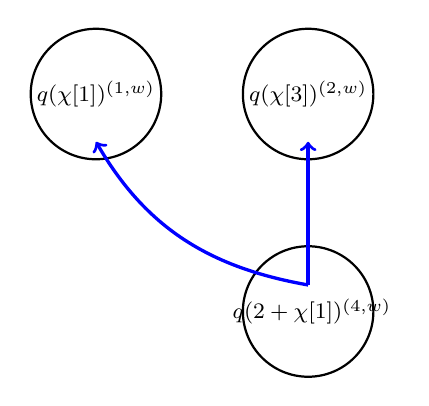
\begin{tikzpicture}[scale=\textwidth/18cm,samples=200]
%%% The nodes represents the k query in the first round
\draw[thick] (2, 4.1) circle (35pt) 
node {\footnotesize{$q(\chi[1])^{(1,w)}$}} ;
\draw[thick] (6, 4.1) circle (35pt) node
{\footnotesize{$q(\chi[3])^{(2,w)}$}};
\draw[thick] (6, 0) circle (35pt) node {\footnotesize{ $q(2+\chi[1])^{(4,w)}$}};
\draw[very thick,->, blue] (6, 0.5)  -- (6, 3.2) ;
\draw[very thick,->, blue] (6, 0.5)  to [out=170,in=300]  (2, 3.2) ;
\end{tikzpicture}
}
}
\]
}    
 

% adaptivity definition - longest path
Finally, we reach the definition of adaptivity, by means of the query-based dependency graph. 

\begin{defn}[Adaptivity in {loop} language]
Given a program $c$, and a memory $m$, a database $D$, a starting loop map $w$, the adaptivity of the dependency graph $G(c, D,m,w) = (V, E)$ is the length of the longest path in this graph. We denote the path from $q({v_q})^{(l,w)}$ to $q({v_q}')^{(l',w')}$ as $p(q({v_q})^{(l,w)}, q({v_q}')^{(l',w')} )$. The adaptivity denoted as $A(c, D, m, w)$.
%
$$A(c, D, m, w) = \max\limits_{q({v_q})^{(l,w)},q({v_q}')^{(l',w')} \in V } |p(q({v_q})^{(l,w)}, q({v_q}')^{(l',w')} )| $$
\end{defn}

% \subsection{ Adaptivity through an example }

%  We still use the two round example in Figure~\ref{fig:simpl-two-round-graph} to illustrate the process of collecting the trace, building the dependency graph and reaching the adaptivity. 

% \[
% TRC(k) \triangleq
% {
% \begin{array}{l}
%     % \left[j \leftarrow 0 \right]^1 ; \\
%   \clabel{ a \leftarrow []}^{1} ; \\
%     \clabel{\assign{j}{0} }^{2} ; \\
%     \eloop ~ \clabel{k}^{3} ~ \edo ~ \\
%     \Big(
%      \clabel{x \leftarrow q(\chi(j)\cdot \chi(k)) }^{4}  ; \\
%      \clabel{\assign{j}{j+1}}^{5} ;\\
%     \clabel{a \leftarrow x :: a}^{6}       \Big);\\
%     \clabel{l \leftarrow q(\mathrm{sign}\big (\sum_{i\in [k]} \chi(i)\times\ln\frac{1+a[i]}{1-a[i]} \big ))}^{7}\\
% \end{array} 
% }
% \]
% \\
% Given a specific database $D = [[1, 1], [0, 0], [1, 1], [1, 1]]$, supposing $a= q_1(\chi[0])(D) +q_1(\chi[1])(D) +q_1(\chi[2])(D) = n$, $n$ is a constant variable $a$ stores in the resulting memory, then the execution trace $t$ is generated along with the operational semantics as follows:
% \\
% $\config{[], TRC(3), D, []>} \to^{*}
% \config{[j \to 3, a \to [1, 0, 1], l \to 1], D, \eskip, t>}$\\
% \[t = \left\{
% q_1(\chi(0))^{(4, [3:1])}, \
% q_1(\chi(1))^{(4, [3:2])}, \ 
% q_1(\chi(2))^{(4, [3:3])}, \ 
% q_2(\chi[4]+n)^{(7, \emptyset)}
% \right \}\]
% For the sake of brevity, we use $q_1(0), q_1(1), q_1(2)$ to represent 
% $ q_1(\chi(0)), 
% q_1(\chi(1)),
% q_1(\chi(2))$. The graph is also shown in Figure~\ref{fig:simpl-two-round-graph}.  


% Then we have the graph as:
% \\
% $V = \left\{
% q_2^6, q_1^{(3,1)}, q_1^{(3,2)}, q_1^{(3,3)}
% \right\}$
% \\
% $E = \left \{
% (q_2^6, q_1^{(3,1)}),
% (q_2^6, q_1^{(3,2)}),
% (q_2^6, q_1^{(3,3)})
% \right\}$
% Then we have the dependency graph generated in Figure \ref{fig:two-round-graph}. 
% \\
% $V = \left\{
% q_{1}(0, 3)^{(3, [1])}, \
% q_{1}(1, 3)^{(3, [2])}, \ 
% q_{1}(2, 3)^{(3, [3])}, \ 
% q_{2}([1, 0, 1])^{(6, [])}
% \right \}$

% Todo: A graph for two round algorithm
% \begin{figure}
% %\begin{figure}
% \begin{tikzpicture}[scale=\textwidth/30cm,samples=200]
% %%% The nodes represents the k query in the first round
% \filldraw[black] (0, 4) circle (5pt) node [anchor=south]{$q_0^{(3,[3:1])}$};
% \filldraw[black] (6, 4) circle (5pt) node [anchor=south]{$q_1^{(3,[3:2])}$};
% \filldraw[black] (12, 4) circle (5pt) node [anchor=south]{$q_2^{(3,[3:3])}$};
% \filldraw[black] (6, 0) circle (5pt) node [anchor=north]{$q(v)^{(7,\emptyset)}$};
% \draw[very thick,->, blue] (6, 0)  -- (6, 3.9) ;
% \draw[very thick,->, red] (6, 0)  -- (12, 3.9) ;
% \draw[very thick,->, blue] (6, 0)  -- (0, 3.9) ;
% \end{tikzpicture}
% \caption{A query-based dependency graph for two round algorithm complete version}
% \label{fig:two-round-graph}
% \end{figure}
%\end{figure}
% Even though the high level loop language provides necessary information for static analysis on most real-world data analysis algorithms, it is not suitable to conduct a static analysis directly on. To be specific, it is challenging to achieve a formal definition of the number of rounds of adaptivity for algorithms using the high level language due to the characteristics depicted in its syntax: the execution of one query $q(e)$ in a program $p$ is decided not only by its explicit control flow (e.g. if statement), but also by its argument $e$. 
%
% Then we have the adaptivity calculated from the graph as:
% \[
% \begin{array}{ll}
% A^*(TR, D, m, w) & = \max\limits_{q(v)^{(l,w)},q'(v')^{(l',w')} \in V }\{ |p(q(v)^{(l,w)}, q'(v')^{(l',w')} )| \}\\
% & = |p(q_2^6, q_1^{(3,3)})| = |p(q_2^6, q_1^{(3,1)})| = |p(q_2^6, q_1^{(3,2)})|\\
% & = 1
% \end{array}
% \]
% We can notice the complete version generates the similar query-based dependency graph as its simplified version in Figure~\ref{fig:simpl-two-round-graph}.

